\documentclass[12pt]{article}
\usepackage[margin=1in]{geometry}
\usepackage{tikz}
\usetikzlibrary{shapes.geometric, arrows, positioning}
% For all the diagram setups
\tikzset{trapezium stretches=true}
\tikzstyle{source} = [rectangle, rounded corners, minimum width= 2cm, minimum height = 1cm, text = white, text centered, fill = black!60]
\tikzstyle{input} = [trapezium, trapezium left angle=50, trapezium right angle = 130, minimum width = 1.5cm, minimum height=1cm, text centered, text=white, fill=green!60!black]
\tikzstyle{routing} = [diamond, minimum width=2cm, minimum height=1cm, aspect = 2, text width = 2cm, text centered, text=white,fill = blue!70!black]
\tikzstyle{processor} = [rectangle, minimum width = 2cm, minimum height = 1cm, text width = 3cm, text = white, fill = purple!55!blue!40!black]
\tikzstyle{cable} = [thick, ->, >=latex]
\tikzstyle{usb} = [thick, <->, >=latex]

\renewcommand{\familydefault}{\sfdefault} %sans font for computer screens

\begin{document}
\centering
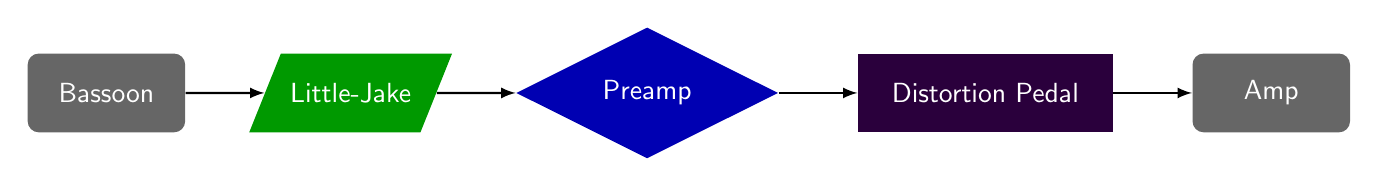
\begin{tikzpicture}[align=center, node distance=1cm]
  \node (bsn) [source] {Bassoon};
  \node (lj) [input, right = of bsn] {Little-Jake};
  \node (preamp) [routing, right = of lj] {Preamp};
  \node (dist) [processor, right = of preamp] {Distortion Pedal};
  \node (amp) [source, right = of dist] {Amp};
  \draw [cable] (bsn) -- (lj);
  \draw [cable] (lj) -- (preamp);
  \draw [cable] (preamp) -- (dist);
  \draw [cable] (dist) -- (amp);
\end{tikzpicture}

\end{document}